% --- Applications (from sections/diffusion/complete/applications.tex) ---
\section{Applications}
\begin{frame}{}
    \LARGE Diffusion Models: \textbf{Applications}
\end{frame}

\begin{frame}[allowframebreaks]{Application: Stable Video Diffusion}
    \begin{itemize}
        \item Initialize from Stable Diffusion.
        \item Add temporal layers (e.g., 1D Conv, temporal attention).
        \item Finetune on video data.
        \item Data pipeline:
        \begin{itemize}
            \item Scrape \textbf{unlabeled} videos from the internet.
            \item Use image and video captioners to generate synthetic text labels.
            \item Apply aggressive data filtering using several heuristics (CLIP score, optical flow score, aesthetic scores, OCR, etc.).
        \end{itemize}
    \end{itemize}
    
    \framebreak

    \begin{figure}
        \centering
        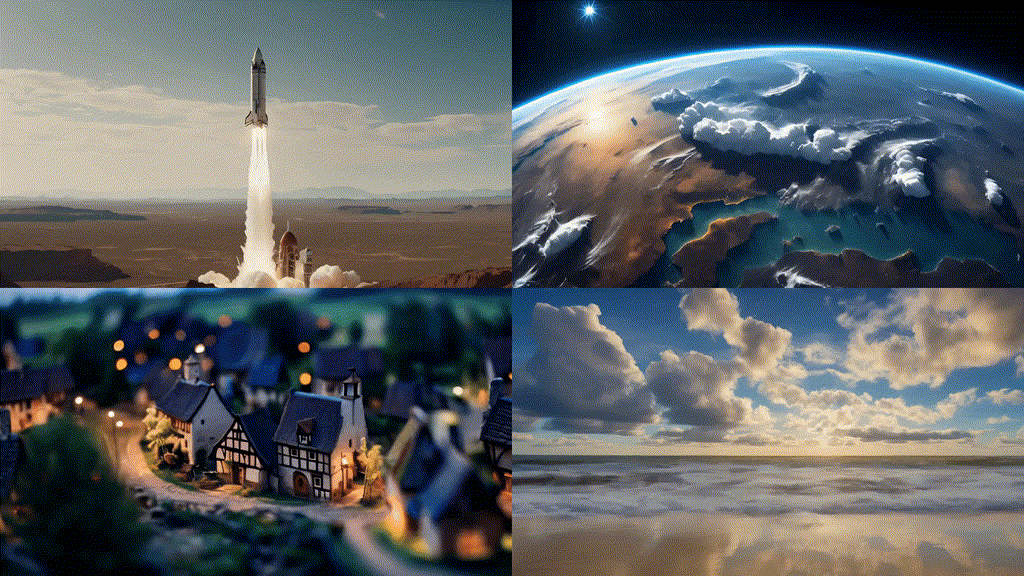
\includegraphics[width=1.06\linewidth,height=\textheight,keepaspectratio]{images/adv-img-gen/slide_101_1_img.png}
        \caption*{\href{https://drive.google.com/file/d/19XVG5MpxMRXP1hwHETkP_prlbHOcuTSj/view?usp=sharing}{Link: GIFF}}
    \end{figure}

\end{frame}

% --- GLIDE (from sections/diffusion/complete/applications/glide.tex) ---
\begin{frame}{Application: GLIDE - OpenAI}
\begin{figure}
    \centering
    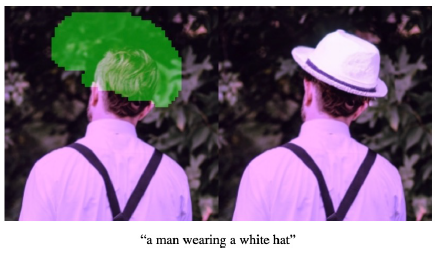
\includegraphics[height=0.8\textheight, width=\textwidth, keepaspectratio]{images/diffusion/diff_results_2.png}
    \caption*{Image Inpainting with GLIDE}
\end{figure}
\footnotetext{\href{https://arxiv.org/abs/2112.10741}{GLIDE: Towards Photorealistic Image Generation and Editing with Text-Guided Diffusion Models}}
\end{frame}

% --- DALL·E 2 (from sections/diffusion/complete/applications/dalle2.tex) ---
\begin{frame}{Application: DALL.E 2 - OpenAI}
\begin{figure}
    \centering
    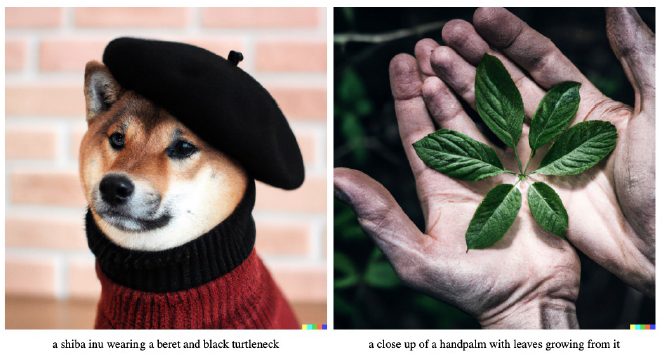
\includegraphics[height=0.8\textheight, width=\textwidth, keepaspectratio]{images/diffusion/diff_results_3.png}
    \caption*{Text to image generation eith DAll.E 2}
\end{figure}
\footnotetext{\href{https://arxiv.org/abs/2204.06125}{Hierarchical Text-Conditional Image Generation with CLIP Latents}}
\end{frame}

\begin{frame}{DALL.E 2 - OpenAI}
\begin{figure}
    \centering
    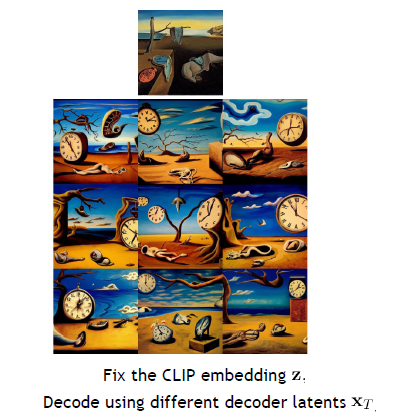
\includegraphics[height=0.8\textheight, width=\textwidth, keepaspectratio]{images/diffusion/diff_results_4.png}
    \caption*{Image Variations}
\end{figure}

\footnotetext{\href{https://arxiv.org/abs/2204.06125}{Hierarchical Text-Conditional Image Generation with CLIP Latents}}


\end{frame}

\begin{frame}{DALL.E 2 - OpenAI}
\begin{figure}
    \centering
    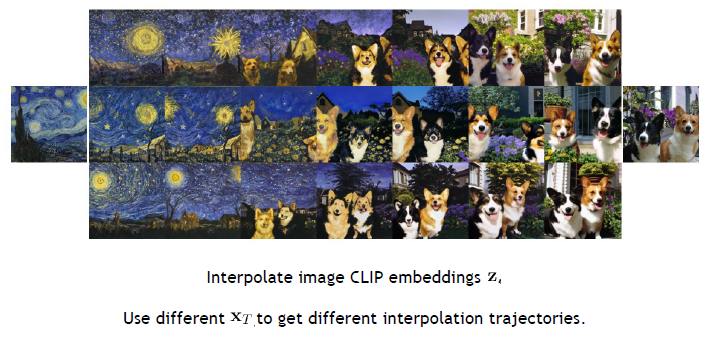
\includegraphics[height=0.8\textheight, width=\textwidth, keepaspectratio]{images/diffusion/diff_results_5.png}
    \caption*{Image interpolation}
\end{figure}

\footnotetext{\href{https://arxiv.org/abs/2204.06125}{Hierarchical Text-Conditional Image Generation with CLIP Latents}}

\end{frame}

\begin{frame}{DALL.E 2 - OpenAI}
\begin{figure}
    \centering
    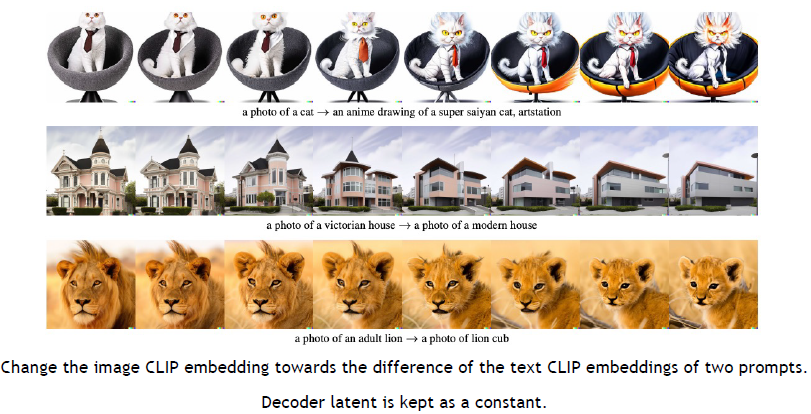
\includegraphics[height=0.8\textheight, width=\textwidth, keepaspectratio]{images/diffusion/diff_results_6.png}
    \caption*{Text Difference Image interpolation}
\end{figure}

\footnotetext{\href{https://arxiv.org/abs/2204.06125}{Hierarchical Text-Conditional Image Generation with CLIP Latents}}

\end{frame}

% --- Imagen (from sections/diffusion/complete/applications/imagen.tex) ---
\begin{frame}{Imagen - Google}

\begin{figure}
    \centering
    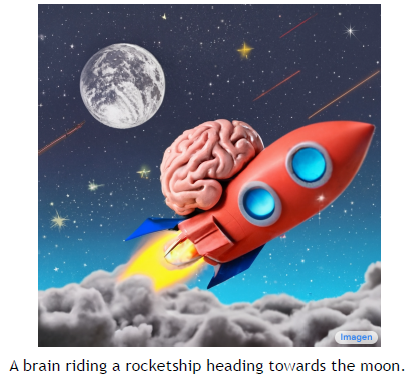
\includegraphics[height=0.8\textheight, width=\textwidth, keepaspectratio]{images/diffusion/diff_results_7.png}
\end{figure}

\footnotetext{\href{https://arxiv.org/abs/2205.11487}{Photorealistic Text-to-Image Diffusion Models with Deep Language Understanding}}
\end{frame}

\begin{frame}{Imagen - Google}

\begin{figure}
    \centering
    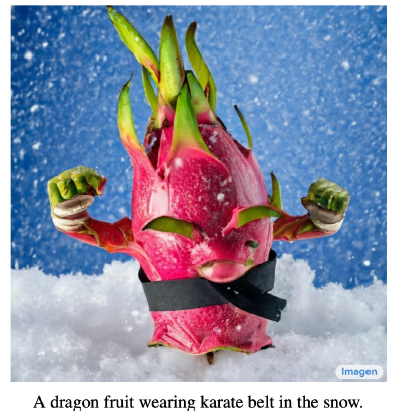
\includegraphics[height=0.8\textheight, width=\textwidth, keepaspectratio]{images/diffusion/diff_results_8.png}
\end{figure}

\footnotetext{\href{https://arxiv.org/abs/2205.11487}{Photorealistic Text-to-Image Diffusion Models with Deep Language Understanding}}
\end{frame}

\begin{frame}{Imagen - Google}

\begin{figure}
    \centering
    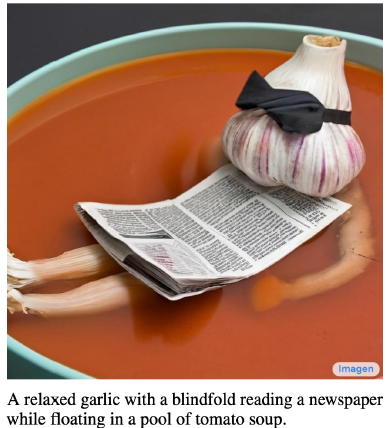
\includegraphics[height=0.8\textheight, width=\textwidth, keepaspectratio]{images/diffusion/diff_results_9.png}
\end{figure}

\footnotetext{\href{https://arxiv.org/abs/2205.11487}{Photorealistic Text-to-Image Diffusion Models with Deep Language Understanding}}
\end{frame}

% --- Stable Diffusion 2.0 (Stability AI blog, Nov 2022) ---
\begin{frame}{Application: Stable Diffusion 2.0}
  \footnotesize
  \textbf{What changed vs.\ Stable Diffusion v1?}
  \begin{itemize}\itemsep0.3em
    \item \textbf{New text encoder:} OpenCLIP (LAION + Stability AI) replaces CLIP ViT-L/14---stronger language understanding and image quality.
    \item \textbf{Native resolutions:} text-to-image at \textbf{512$\times$512} and \textbf{768$\times$768}.
    \item \textbf{Upscaler diffusion:} $\times 4$ super-resolution (e.g.\ 128$\rightarrow$512).
    \item \textbf{depth2img:} depth-guided image-to-image---structure-preserving synthesis from inferred depth + text.
    \item \textbf{Updated inpainting:} text-guided inpainting fine-tuned on the Stable Diffusion 2.0 base model.
  \end{itemize}
  \footnotetext{\href{https://stability.ai/news-updates/stable-diffusion-v2-release}{Lopez, ``Stable Diffusion 2.0 Release,'' Stability AI (Nov 2022).}}
\end{frame}

\begin{frame}{Stable Diffusion 2.0: Upscaler Diffusion}
  \begin{columns}[T,onlytextwidth]
    \column{0.44\textwidth}
      \footnotesize
      \begin{itemize}\itemsep0.35em
        \item Dedicated \textbf{upscaler diffusion} model enhances resolution by \textbf{$\times 4$}.
        \item Example: \textbf{128$\times$128} low-res sample $\rightarrow$ \textbf{512$\times$512} output.
      \end{itemize}
    \column{0.54\textwidth}
      \centering
      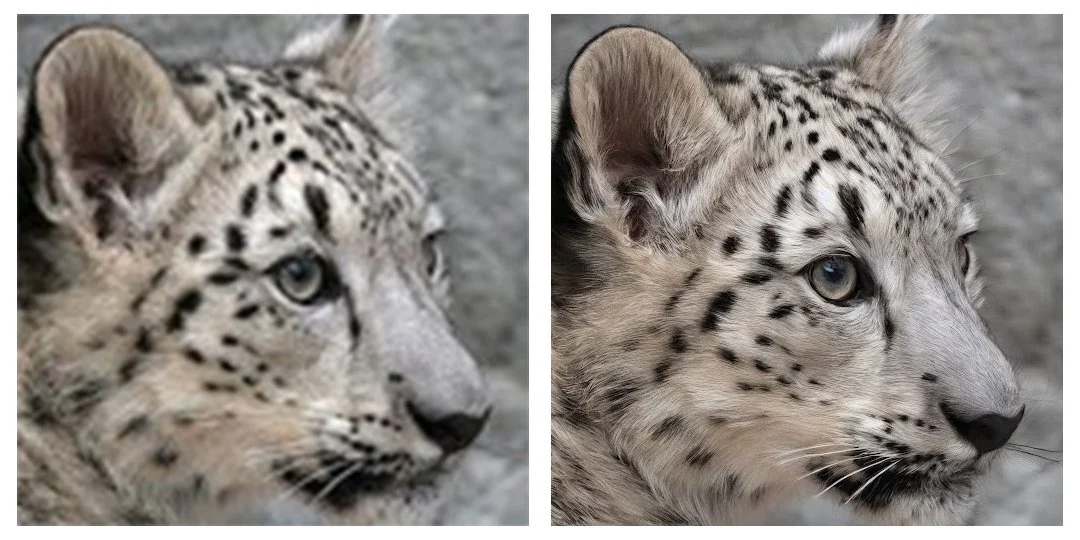
\includegraphics[width=\linewidth,height=0.68\textheight,keepaspectratio]{assets/New-Lecture-Stable_Diffusion/sd2/upscaler_crop.png}\\[0.15em]
      {\scriptsize Left: 128$\times$128.\quad Right: 512$\times$512 upscaled.}
  \end{columns}
  \footnotetext{\href{https://stability.ai/news-updates/stable-diffusion-v2-release}{Stability AI, Stable Diffusion 2.0 Release.}}
\end{frame}

\begin{frame}{Stable Diffusion 2.0: depth2img}
  \begin{columns}[T,onlytextwidth]
    \column{0.48\textwidth}
      \begin{itemize}\itemsep0.35em
        \item \textbf{depth2img} infers depth from an input image, then generates new images conditioned on \textbf{text + depth}.
        \item Enables structure-preserving image-to-image and shape-conditional synthesis.
        \item Can produce radically different appearances while preserving spatial coherence and depth.
      \end{itemize}
    \column{0.50\textwidth}
      \centering
      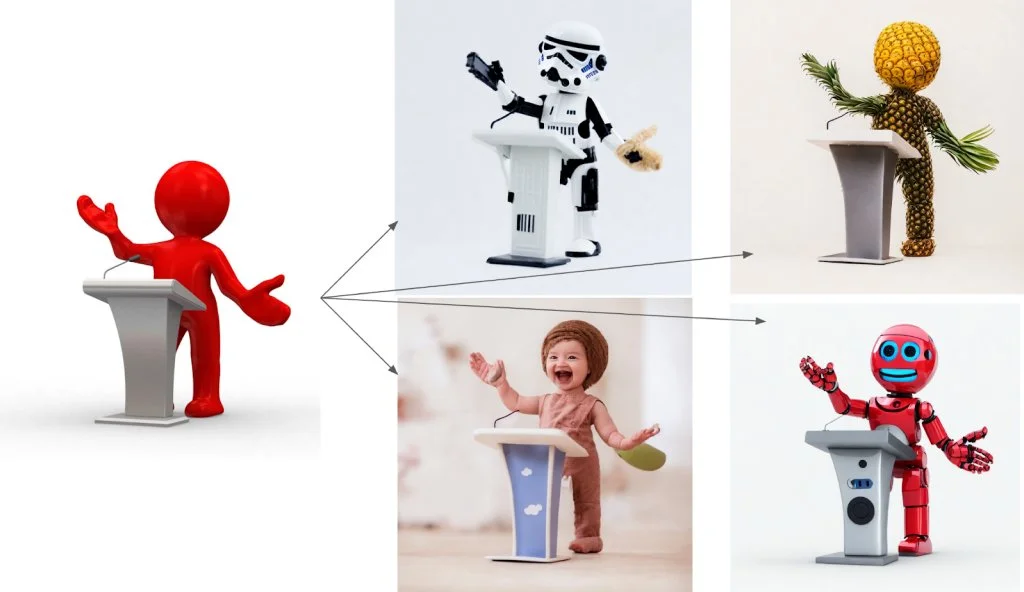
\includegraphics[width=\linewidth,height=0.34\textheight,keepaspectratio]{assets/New-Lecture-Stable_Diffusion/sd2/depth2img_crop.png}\\[0.2em]
      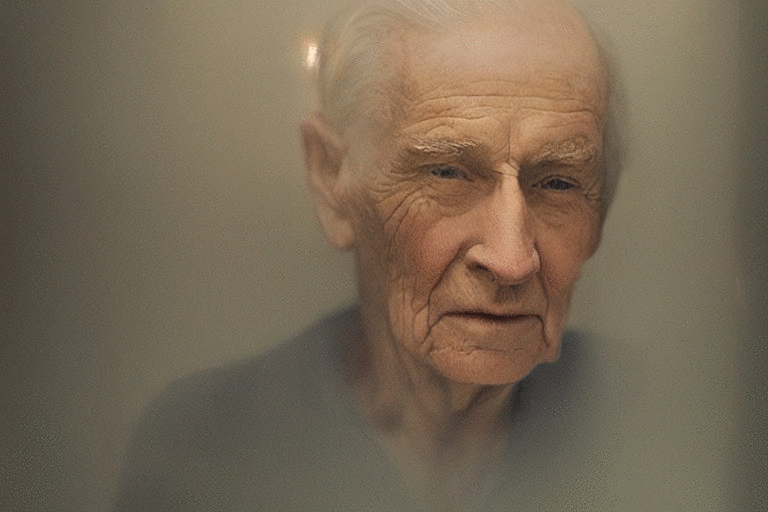
\includegraphics[width=\linewidth,height=0.34\textheight,keepaspectratio]{assets/New-Lecture-Stable_Diffusion/sd2/depth2img_coherence_frame0.png}\\[0.1em]
      {\scriptsize Input $\rightarrow$ variants (top); depth coherence preserved (bottom).}
  \end{columns}
  \footnotetext{\href{https://stability.ai/news-updates/stable-diffusion-v2-release}{Stability AI, Stable Diffusion 2.0 Release.}}
\end{frame}

\begin{frame}{Stable Diffusion 2.0: Inpainting}
  \centering
  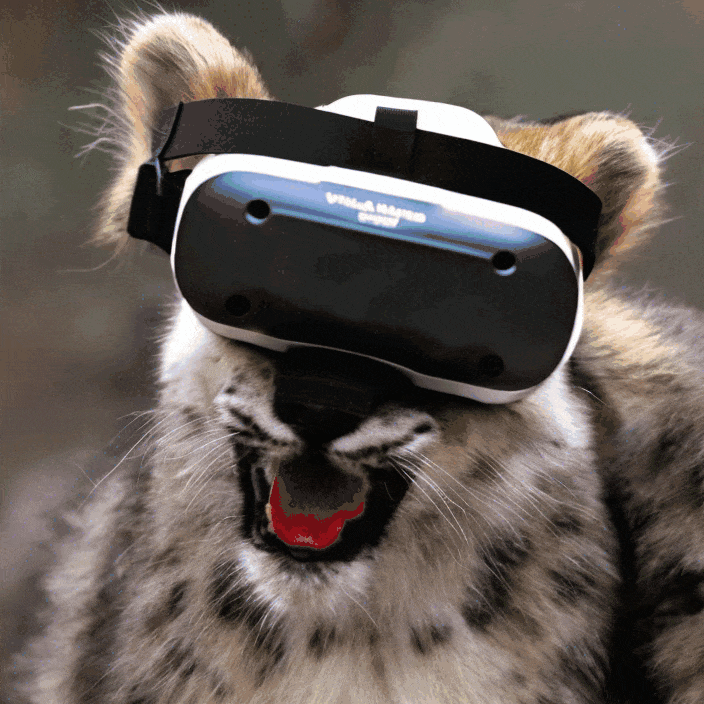
\includegraphics[width=0.62\linewidth,height=0.72\textheight,keepaspectratio]{assets/New-Lecture-Stable_Diffusion/sd2/inpainting_frame0.png}\\[0.2em]
  {\scriptsize Text-guided inpainting model fine-tuned on the SD~2.0 text-to-image base.}
  \footnotetext{\href{https://stability.ai/news-updates/stable-diffusion-v2-release}{Stability AI, Stable Diffusion 2.0 Release.}}
\end{frame}

% --- Stable Diffusion 3.5 (Stability AI blog, Oct 2024) ---

% \begin{frame}[allowframebreaks]{Application: Stable Diffusion 3.5}
%   \vspace{0.4em}
%   \centering
%   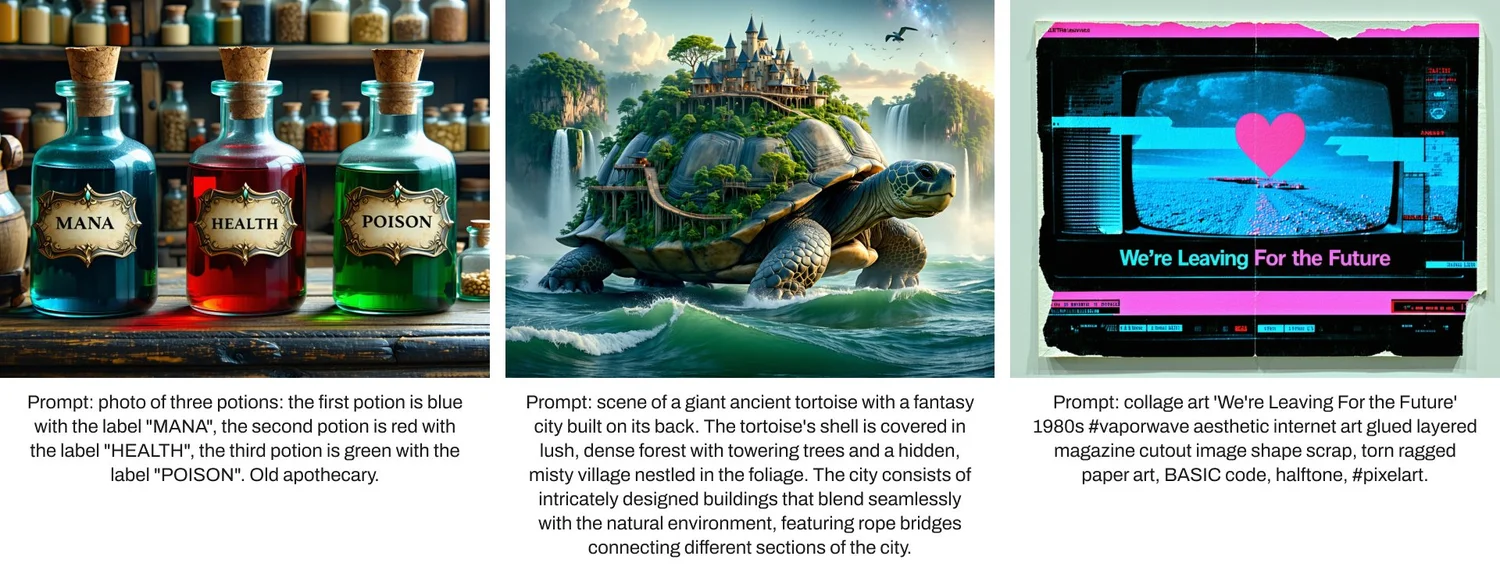
\includegraphics[width=\linewidth,height=0.38\textheight,keepaspectratio]{assets/New-Lecture-Stable_Diffusion/sd35/benchmark_medium_crop.png}
%   \footnotetext{\href{https://stability.ai/news-updates/introducing-stable-diffusion-3-5}{Stability AI, ``Introducing Stable Diffusion 3.5'' (Oct 2024).}}
% \end{frame}

\begin{frame}{Stable Diffusion 3.5: Diverse \& Versatile Outputs}
    \centering
    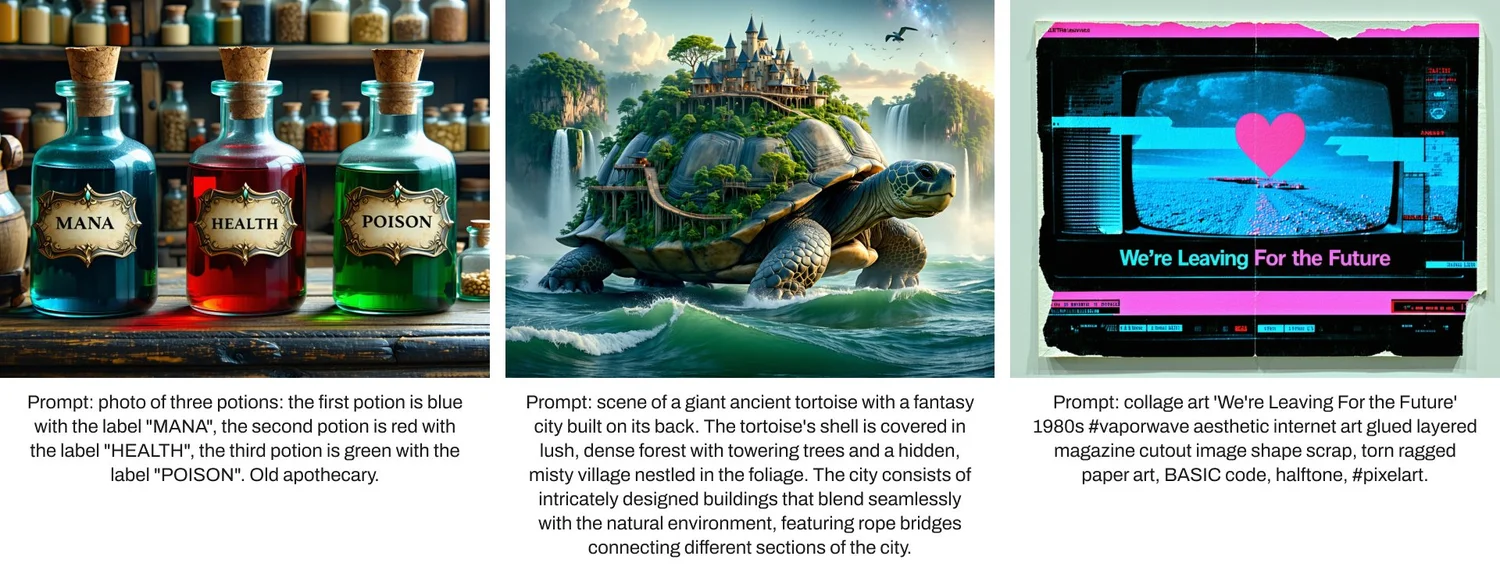
\includegraphics[width=\linewidth,height=0.38\textheight,keepaspectratio]{assets/New-Lecture-Stable_Diffusion/sd35/benchmark_medium_crop.png}
      \begin{itemize}\itemsep0.35em
        \item \textbf{Customizability:} Large (8.1B), Large Turbo (8.1B) and Medium (2.5B) models.
        \item \textbf{Efficient Performance:} Optimized to run on standard consumer hardware; Medium and Large Turbo require no specialized GPUs.
        \item \textbf{Highly Accessible:} Medium needs only 9.9GB of VRAM making advanced diffusion imaging feasible on most consumer GPUs.
      \end{itemize}
\end{frame}

% --- Nano Banana 2 (Google DeepMind blog, Feb 2026) ---
\begin{frame}[t]{Application: Nano Banana 2 -- Google DeepMind}
    \begin{figure}
        \centering
        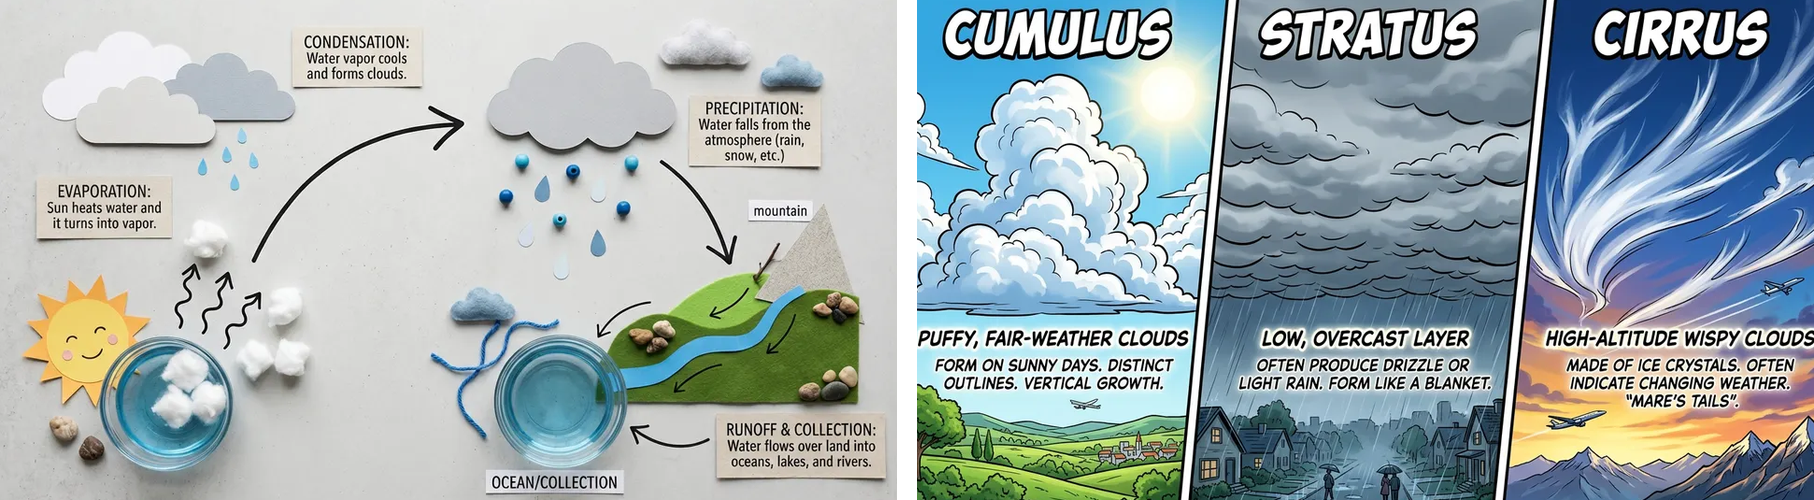
\includegraphics[width=\linewidth,keepaspectratio]{assets/New-Lecture-Stable_Diffusion/nano-banana-2/slide1_world_knowledge.png}
        \caption*{Examples: water-cycle infographic and cloud-type comparison.}
    \end{figure}
    \footnotetext{\href{https://blog.google/innovation-and-ai/technology/ai/nano-banana-2/}{Raisinghani, ``Nano Banana 2: Combining Pro capabilities with lightning-fast speed,'' Google DeepMind blog (Feb 2026).}}
    \begin{itemize}
        \item Builds on Google's Gemini Image line: Nano Banana (2025) $\rightarrow$ Nano Banana Pro $\rightarrow$ Nano Banana 2.
        \item Production-ready output: multiple aspect ratios and resolutions from 512px to 4K.
    \end{itemize}
\end{frame}

\begin{frame}{Try It Yourself!}
\centering
Text to Image generation with stable diffusion.
\centering
\href{https://huggingface.co/spaces/stabilityai/stable-diffusion}{https://huggingface.co/spaces/stabilityai/stable-diffusion}

\footnotetext{\href{https://arxiv.org/abs/2112.10752}{High-Resolution Image Synthesis with Latent Diffusion Models}}
\end{frame}
